\documentclass[a4paper,12pt]{article}
\usepackage{graphicx}
\usepackage{titlesec}
\usepackage[utf8]{inputenc}
\usepackage{xcolor}
\usepackage{fancyhdr}
\usepackage{lipsum}
\usepackage{caption}

\renewcommand{\headrulewidth}{0pt}
\fancyhead[C]{}
\fancyhead[C]{
	
\includegraphics[width=4cm]{metu}
}
\pagestyle{plain}

%opening
\title{Middle East Technical University\\Department of Physics\\\textbf{PHYS307 Applied Modern Physics}}
\author{Oğuzhan ÖZCAN\\}
\date{}
\clearpage
\thispagestyle{empty}
\providecommand{\groupmember}[1]{\textbf{Group Members:} }
\providecommand{\expdate}[1]{\textbf{Experiment Date:} }
\providecommand{\repdate}[1]{\textbf{Report Submit Date:} }
\providecommand{\expname}[1]{\textbf{Exp. MP-AG The Absorption of Gamma Rays} }


\usepackage[a4paper,%
left=0.5in,right=0.5in,top=0.5in,bottom=0.8in,%
footskip=.25in]{geometry}
%\topmargin -4.5cm
%\oddsidemargin 0.2cm
%\textwidth 16cm %
%\textheight 21cm%
%\footskip 1.0cm%




\begin{document}
\pagenumbering{gobble}
\maketitle

\thispagestyle{fancy}

%%%%%%%%%%%%%%%%%%%%%%%%%%%%%%%%%%%%%%%%%%%%%%%%%%%%%
\noindent\rule{18.4cm}{0.8pt}
\begin{center}
	\expname{arg1}{}
\end{center}


\noindent\rule{18.4cm}{0.8pt}\\\\
%%%%%%%%%%%%%%%%%%%%%%%%%%%%%%%%%%%%%%%%%%%%%%%%%%%%%
\begin{table}[h!]
\begin{center}
	\begin{tabular}{|c|c|c|c|}
	\hline Trial 1 & Trial 2 & Trial 3  & Average \\ 
	\hline 1932 & 1831 & 1914 & 1892 \\ 
	\hline 
\end{tabular}
\end{center}
\caption{Background Intensity [counts/min]} 
\end{table}
\begin{figure}[h!]
\centering
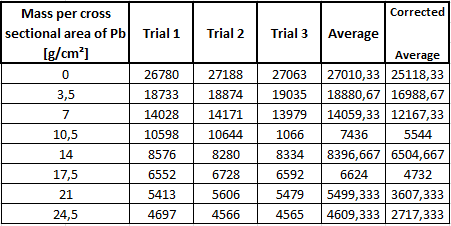
\includegraphics[scale = 1.0]{Capture}
\caption{Counting rates of radiation from $^{137}$Cs for different thickness of lead}
\label{fig:Capture}
\end{figure}

Slope of the line = 21759e$^{-0.088x}$\\
Mass absorption coefficient $\mu_{m}$ = 7.76$\times 10^{-3}$ cm$^{2}$/g\\
Linear absorption coefficient $\mu$ = 0.088 cm$^{-1}$\\
Apparent energy value of $\gamma$-rays from $^{137}$Cs = 667.0 keV\\
Accepted energy value of $\gamma$-rays from $^{137}$Cs obtained from Fig.AG.1 = 661.6 keV \\
Percentage error in the energy of $\gamma$-rays from $^{137}$Cs = 0.81 \%
\newpage
\textbf{1. What is the half thickness of $\gamma$-rays from $^{137}$Cs in lead?}\\\\
The half thickness $d_{1/2}$ of a material is the thickness that decreases the incident radiation energy by one half. We can express this quantity as follows 
\begin{equation}
d_{1/2}=\frac{\ln 2}{\mu }
\end{equation}
As we stated above $\mu$ is 0.088 cm$^{-1}$. So
\begin{equation}
d_{1/2}=\frac{\ln 2}{0.088}
\end{equation}
\begin{equation}
d_{1/2}=7.87 cm
\end{equation}
\textbf{2. Compute the percent of an incident beam of $\gamma$-rays from $^{137}$Cs after passing through 2 mm of lead.}
\begin{equation}
I=I_{0}e^{-\mu x}
\end{equation}
$\mu$=0.088 cm$^{-1}$, $x$ is 0.20 cm, $\rho_{Pb}=11.3 g/cm^{3}$

\begin{equation}
\frac{I}{I_{0}}=e^{-\mu x}=e^{-0.088\times 0.20}
\end{equation}
\begin{equation}
\frac{I}{I_{0}}=e^{-0.0176}
\end{equation}
\begin{equation}
\frac{I}{I_{0}}=0.98
\end{equation}
above results show that the transmitted beam. Therefore \%2 of the beams is absorbed.
\newpage
\textbf{3. Would the semilog graph of intensity versus thickness of the absorber be a straight line if the $\gamma$-radiation contained $\gamma$-rays of two different energies? Explain.}\\\\
\begin{figure}[h!]
\centering
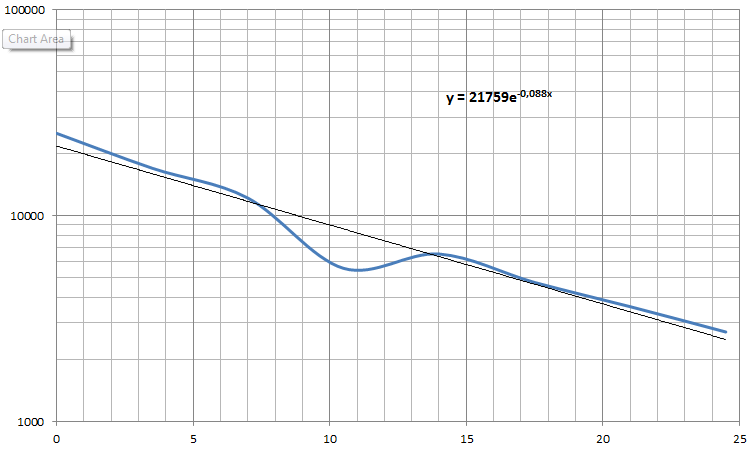
\includegraphics[scale = 0.8 ]{plot1}
\caption{Graph of Intensity versus Thickness of the Absorber }
\label{fig:plot1}
\end{figure}

No, if there were two absorption coefficients, Eq. 4 would have the form of 
\begin{equation}
I=I_{1}e^{-\mu_{1}x}+I_{2}e^{-\mu_{2}x}
\end{equation}
When the logarithms of both sides are taken, this does not reduce to a straight line.\\\\
\textbf{4. The mass absorption coefficient of iron is 0.058 cm$^{2}$/g for 1.24 MeV $\gamma$-rays. What percentage of the beam of such $\gamma$-rays is transmitted (if any) through an iron plate 3 cm thick? ($\rho_{Fe}$=7.86g/cm$^{2}$)}\\\\
$\mu_{m}$=0.058 cm$^{2}$/g, x=3 cm, $\rho_{Fe}=7.86$ g/cm$^{3}$\\
\begin{equation}
\mu=\rho_{Fe}\mu_{m}=7.86\times 0.058=0.46 cm^{-1}
\end{equation}
\begin{equation}
\frac{I}{I_{0}}=e^{-\mu x}=e^{0.46\times 3}=e^{-1.38}=0.25=25\%
\end{equation}

\newpage
\textbf{Discussion and Conclusion}\\\\
The absorption of nuclear radiation is important in many applications. In this experiment we measured the gamma rays in different thickness. As we expect before the experiment, decreasing in thickness of lead causes to decrease in counting rates of gamma radiation. We used Cesium-137 ($^{137}$Cs) which is a good beta-gamma radiation source. According to our results, we can state that gamma ray intensity decays exponentially with the thickness of the material.







































































































































\end{document}
